% CAP description for Tree
A Tree is a component with linked
elements (nodes) and a hierarchical structure. One common example is
the display of directory structures used in most file managers
(e.g. \bxname{Windows Explorer}).

\begin{figure}
\begin{center}
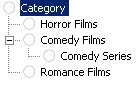
\includegraphics{PS/Tree}
\caption{Tree}
\label{tree}
\end{center}
\end{figure}

\textbf{Mapping trees}

In the \gdomm{}, a tree to be mapped looks like this:

\begin{figure}
\begin{center}
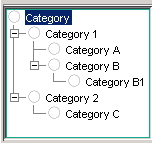
\includegraphics{PS/Maptree}
\caption{Tree}
\label{maptree}
\end{center}
\end{figure}